% J. R. Capablanca - E. A. Snosko-Borovski, St. Petersburg, 1913, with Capablanca's notes.
% Build with: python3 ../../tools/chessbook.py game-04-capablanca-snosko-borovski.tex
\documentclass[10pt,twoside]{article}
\usepackage[paperwidth=487.56bp,paperheight=691.65bp,top=72pt,bottom=44pt,inner=50pt,outer=48pt,
            headheight=13pt,headsep=20pt,footskip=0pt]{geometry}
\usepackage[T1]{fontenc}
\usepackage[lining]{ebgaramond}
\usepackage{graphicx}
\usepackage{microtype}
\usepackage{tikz}
\usepackage{fancyhdr}
\usepackage[hidelinks,pdftitle={Capablanca - Snosko-Borovski, St. Petersburg, 1913},
            pdfauthor={J. R. Capablanca}]{hyperref}

\newcommand{\textsizebook}{\fontsize{10.5}{12.6}\selectfont}
\AtBeginDocument{\textsizebook}
\setlength{\columnsep}{11pt}
\setlength{\parindent}{9pt}
\setlength{\parskip}{0pt}
\setlength{\emergencystretch}{1.5em}
\raggedbottom

\newlength{\boardwidth}
\setlength{\boardwidth}{160pt}

% A main line move, as a bold heading above its note
\newcommand{\Move}[1]{\par\addvspace{8pt}\noindent\phantomsection{\bfseries #1}\par\nopagebreak}
% A diagram in the text
\newcommand{\ChessDiagram}[1]{\par\addvspace{7pt}{\centering #1\par}\addvspace{5pt}}

\pagestyle{fancy}
\fancyhf{}
\renewcommand{\headrulewidth}{0pt}
\fancyhead[LE,RO]{\thepage}
\fancyhead[CE]{French Defence}
\fancyhead[CO]{Capablanca -- Snosko-Borovski}






\newcommand{\figK}{\raisebox{-0.14em}{
\includegraphics[height=1em]{diagrams/figK}}}
\newcommand{\figQ}{\raisebox{-0.14em}{
\includegraphics[height=1em]{diagrams/figQ}}}
\newcommand{\figR}{\raisebox{-0.14em}{
\includegraphics[height=1em]{diagrams/figR}}}
\newcommand{\figB}{\raisebox{-0.14em}{
\includegraphics[height=1em]{diagrams/figB}}}
\newcommand{\figN}{\raisebox{-0.14em}{
\includegraphics[height=1em]{diagrams/figN}}}
\begin{document}

\twocolumn[{%
\thispagestyle{empty}
\begin{tikzpicture}[remember picture,overlay]
  \node[circle,draw=black,line width=1.6pt,fill=black!20,minimum size=112pt] (seal)
       at ([xshift=75pt,yshift=-75pt]current page.north west) {};
  \draw[line width=0.9pt] ([shift={(-48pt,-30pt)}]seal.center) -- ([shift={(44pt,34pt)}]seal.center);
  \node[rotate=37] at ([shift={(-11pt,14pt)}]seal.center) {\fontsize{25}{25}\selectfont\bfseries Game};
  \node[rotate=37] at ([shift={(10pt,-16pt)}]seal.center) {\fontsize{38}{38}\selectfont\bfseries 4};
  \node[anchor=north east] at ([xshift=-14pt,yshift=-24pt]current page.north east)
       {\href{https://lichess.org/analysis/pgn/d4_e6_e4_d5_Nc3_Nf6_Bg5_Bb4}{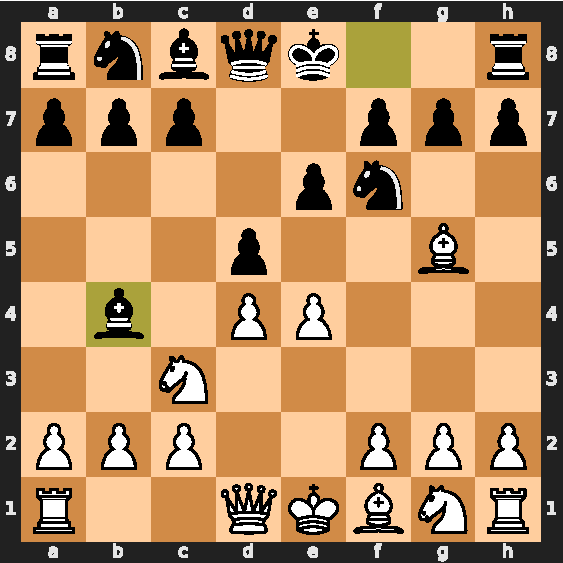
\includegraphics[width=108pt]{diagrams/board-fc02fb03fa03}}};
\end{tikzpicture}

\vspace*{38pt}
\begin{center}
  \begin{minipage}{235pt}\centering
    {\fontsize{22}{25}\selectfont\bfseries French Defence\par}
    \vspace{4pt}\rule{\linewidth}{1pt}\\[-9.5pt]\rule{\linewidth}{0.4pt}
  \end{minipage}

  \vspace{14pt}
  {\fontsize{19}{22}\selectfont\bfseries Capablanca -- Snosko-Borovski\par}
  \vspace{10pt}
  {\fontsize{15}{18}\selectfont\bfseries St. Petersburg, 1913\par}
  \vspace{8pt}
  {\fontsize{11}{13}\selectfont White: J. R. Capablanca \quad Black: E. A. Snosko-Borovski\par}
  \vspace{10pt}
  {\centering\fontsize{8.5}{10}\selectfont\itshape
   Notes by J. R. Capablanca, from \textup{Chess Fundamentals} (1921), which is in the public domain.\\
   Descriptive notation has been converted to algebraic. Page references are to the book.\\
   Click any move or diagram to open it on Lichess.\par}
\end{center}
\vspace{10pt}
}]
\textsizebook

\Move{\href{https://lichess.org/analysis/pgn/d4}{1.d4} \href{https://lichess.org/analysis/pgn/d4_e6}{e6} \href{https://lichess.org/analysis/pgn/d4_e6_e4}{2.e4} \href{https://lichess.org/analysis/pgn/d4_e6_e4_d5}{d5} \href{https://lichess.org/analysis/pgn/d4_e6_e4_d5_Nc3}{3.\figN c3} \href{https://lichess.org/analysis/pgn/d4_e6_e4_d5_Nc3_Nf6}{\figN f6} \href{https://lichess.org/analysis/pgn/d4_e6_e4_d5_Nc3_Nf6_Bg5}{4.\figB g5} \href{https://lichess.org/analysis/pgn/d4_e6_e4_d5_Nc3_Nf6_Bg5_Bb4}{\figB b4}}

This constitutes the \emph{McCutcheon Variation}. It aims at taking the initiative away from White. Instead of defending, Black makes a counter demonstration on the Queen's side. It leads to highly interesting games.

\Move{\href{https://lichess.org/analysis/pgn/d4_e6_e4_d5_Nc3_Nf6_Bg5_Bb4_exd5}{5.exd5}}

At the time this game was played the variation \href{https://lichess.org/analysis/pgn/d4_e6_e4_d5_Nc3_Nf6_Bg5_Bb4_e5}{5.e5} was in vogue, but I considered then, as I do now, the text move to be the stronger.

\Move{\href{https://lichess.org/analysis/pgn/d4_e6_e4_d5_Nc3_Nf6_Bg5_Bb4_exd5_Qxd5}{5...\figQ xd5}}

This is considered superior to \href{https://lichess.org/analysis/pgn/d4_e6_e4_d5_Nc3_Nf6_Bg5_Bb4_exd5_exd5}{5...exd5}. It has for its object, as I said before, to take the initiative away from White by disrupting White's Queen's side. White, however, has more than ample compensation through his breaking up Black's King's side. It might be laid down as a principle of the opening that \emph{the breaking up of the King's side is of more importance than a similar occurrence on the Queen's side}.

\Move{\href{https://lichess.org/analysis/pgn/d4_e6_e4_d5_Nc3_Nf6_Bg5_Bb4_exd5_Qxd5_Bxf6}{6.\figB xf6} \href{https://lichess.org/analysis/pgn/d4_e6_e4_d5_Nc3_Nf6_Bg5_Bb4_exd5_Qxd5_Bxf6_Bxc3}{\figB xc3+} \href{https://lichess.org/analysis/pgn/d4_e6_e4_d5_Nc3_Nf6_Bg5_Bb4_exd5_Qxd5_Bxf6_Bxc3_bxc3}{7.bxc3} \href{https://lichess.org/analysis/pgn/d4_e6_e4_d5_Nc3_Nf6_Bg5_Bb4_exd5_Qxd5_Bxf6_Bxc3_bxc3_gxf6}{gxf6} \href{https://lichess.org/analysis/pgn/d4_e6_e4_d5_Nc3_Nf6_Bg5_Bb4_exd5_Qxd5_Bxf6_Bxc3_bxc3_gxf6_Nf3}{8.\figN f3} \href{https://lichess.org/analysis/pgn/d4_e6_e4_d5_Nc3_Nf6_Bg5_Bb4_exd5_Qxd5_Bxf6_Bxc3_bxc3_gxf6_Nf3_b6}{b6}}

The plan of Black in this variation is to post his Bishop on the long diagonal so as to be able later on, in conjunction with the action of his Rooks along the open g-file, to make a violent attack against White's King. It is, of course, expected that White will Castle on the King's side because of the broken-up condition of his Queen's side Pawns.

\Move{\href{https://lichess.org/analysis/pgn/d4_e6_e4_d5_Nc3_Nf6_Bg5_Bb4_exd5_Qxd5_Bxf6_Bxc3_bxc3_gxf6_Nf3_b6_Qd2}{9.\figQ d2} \href{https://lichess.org/analysis/pgn/d4_e6_e4_d5_Nc3_Nf6_Bg5_Bb4_exd5_Qxd5_Bxf6_Bxc3_bxc3_gxf6_Nf3_b6_Qd2_Bb7}{\figB b7} \href{https://lichess.org/analysis/pgn/d4_e6_e4_d5_Nc3_Nf6_Bg5_Bb4_exd5_Qxd5_Bxf6_Bxc3_bxc3_gxf6_Nf3_b6_Qd2_Bb7_Be2}{10.\figB e2} \href{https://lichess.org/analysis/pgn/d4_e6_e4_d5_Nc3_Nf6_Bg5_Bb4_exd5_Qxd5_Bxf6_Bxc3_bxc3_gxf6_Nf3_b6_Qd2_Bb7_Be2_Nd7}{\figN d7} \href{https://lichess.org/analysis/pgn/d4_e6_e4_d5_Nc3_Nf6_Bg5_Bb4_exd5_Qxd5_Bxf6_Bxc3_bxc3_gxf6_Nf3_b6_Qd2_Bb7_Be2_Nd7_c4}{11.c4} \href{https://lichess.org/analysis/pgn/d4_e6_e4_d5_Nc3_Nf6_Bg5_Bb4_exd5_Qxd5_Bxf6_Bxc3_bxc3_gxf6_Nf3_b6_Qd2_Bb7_Be2_Nd7_c4_Qf5}{\figQ f5} \href{https://lichess.org/analysis/pgn/d4_e6_e4_d5_Nc3_Nf6_Bg5_Bb4_exd5_Qxd5_Bxf6_Bxc3_bxc3_gxf6_Nf3_b6_Qd2_Bb7_Be2_Nd7_c4_Qf5_O-O-O}{12.0--0--0}}

An original idea, I believe, played for the first time in a similar position in a game against Mr. Walter Penn Shipley, of Philadelphia. My idea is that as there is no Black Bishop and because Black's pieces have been developed with a view to an attack on the King's side, it will be impossible for Black to take advantage of the apparently unprotected position of White's King. Two possibilities must be considered. Firstly: If Black Castles on the Queen's side, as in this game, it is evident that there is no danger of an attack. Secondly: If Black Castles on the King's side, White begins the attack first, taking advantage of the awkward position of Black's Queen. In addition to the attacking probabilities of the text move, White in one move brings his King into safety and brings one of his Rooks into play. Thus he gains several moves, ``tempi'' as they are called, which will serve him to develop whatever plan he may wish to evolve.

\Move{\href{https://lichess.org/analysis/pgn/d4_e6_e4_d5_Nc3_Nf6_Bg5_Bb4_exd5_Qxd5_Bxf6_Bxc3_bxc3_gxf6_Nf3_b6_Qd2_Bb7_Be2_Nd7_c4_Qf5_O-O-O_O-O-O}{12...0--0--0} \href{https://lichess.org/analysis/pgn/d4_e6_e4_d5_Nc3_Nf6_Bg5_Bb4_exd5_Qxd5_Bxf6_Bxc3_bxc3_gxf6_Nf3_b6_Qd2_Bb7_Be2_Nd7_c4_Qf5_O-O-O_O-O-O_Qe3}{13.\figQ e3} \href{https://lichess.org/analysis/pgn/d4_e6_e4_d5_Nc3_Nf6_Bg5_Bb4_exd5_Qxd5_Bxf6_Bxc3_bxc3_gxf6_Nf3_b6_Qd2_Bb7_Be2_Nd7_c4_Qf5_O-O-O_O-O-O_Qe3_Rhg8}{\figR hg8} \href{https://lichess.org/analysis/pgn/d4_e6_e4_d5_Nc3_Nf6_Bg5_Bb4_exd5_Qxd5_Bxf6_Bxc3_bxc3_gxf6_Nf3_b6_Qd2_Bb7_Be2_Nd7_c4_Qf5_O-O-O_O-O-O_Qe3_Rhg8_g3}{14.g3} \href{https://lichess.org/analysis/pgn/d4_e6_e4_d5_Nc3_Nf6_Bg5_Bb4_exd5_Qxd5_Bxf6_Bxc3_bxc3_gxf6_Nf3_b6_Qd2_Bb7_Be2_Nd7_c4_Qf5_O-O-O_O-O-O_Qe3_Rhg8_g3_Qa5}{\figQ a5}}

Unquestionably a mistake, overlooking White's fine reply, but a careful examination will show that White already has the better position.

\Move{\href{https://lichess.org/analysis/pgn/d4_e6_e4_d5_Nc3_Nf6_Bg5_Bb4_exd5_Qxd5_Bxf6_Bxc3_bxc3_gxf6_Nf3_b6_Qd2_Bb7_Be2_Nd7_c4_Qf5_O-O-O_O-O-O_Qe3_Rhg8_g3_Qa5_Rd3}{15.\figR d3!} \href{https://lichess.org/analysis/pgn/d4_e6_e4_d5_Nc3_Nf6_Bg5_Bb4_exd5_Qxd5_Bxf6_Bxc3_bxc3_gxf6_Nf3_b6_Qd2_Bb7_Be2_Nd7_c4_Qf5_O-O-O_O-O-O_Qe3_Rhg8_g3_Qa5_Rd3_Kb8}{\figK b8} \href{https://lichess.org/analysis/pgn/d4_e6_e4_d5_Nc3_Nf6_Bg5_Bb4_exd5_Qxd5_Bxf6_Bxc3_bxc3_gxf6_Nf3_b6_Qd2_Bb7_Be2_Nd7_c4_Qf5_O-O-O_O-O-O_Qe3_Rhg8_g3_Qa5_Rd3_Kb8_Rhd1}{16.\figR hd1} \href{https://lichess.org/analysis/pgn/d4_e6_e4_d5_Nc3_Nf6_Bg5_Bb4_exd5_Qxd5_Bxf6_Bxc3_bxc3_gxf6_Nf3_b6_Qd2_Bb7_Be2_Nd7_c4_Qf5_O-O-O_O-O-O_Qe3_Rhg8_g3_Qa5_Rd3_Kb8_Rhd1_Qf5}{\figQ f5}}

\ChessDiagram{\href{https://lichess.org/analysis/pgn/d4_e6_e4_d5_Nc3_Nf6_Bg5_Bb4_exd5_Qxd5_Bxf6_Bxc3_bxc3_gxf6_Nf3_b6_Qd2_Bb7_Be2_Nd7_c4_Qf5_O-O-O_O-O-O_Qe3_Rhg8_g3_Qa5_Rd3_Kb8_Rhd1_Qf5}{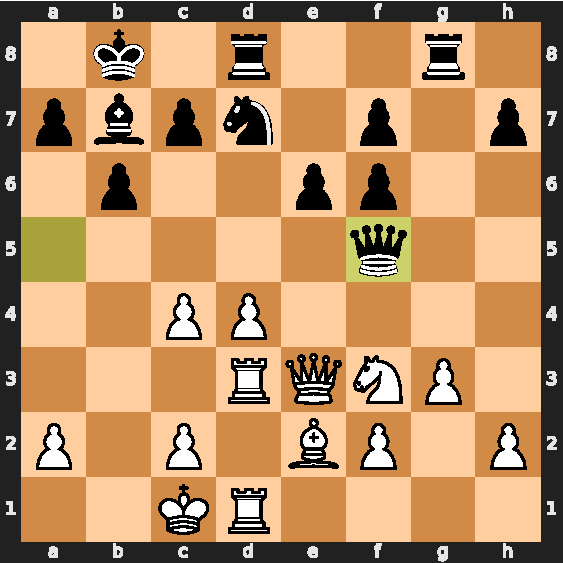
\includegraphics[width=\boardwidth]{diagrams/board-580177624d88}}}

\Move{\href{https://lichess.org/analysis/pgn/d4_e6_e4_d5_Nc3_Nf6_Bg5_Bb4_exd5_Qxd5_Bxf6_Bxc3_bxc3_gxf6_Nf3_b6_Qd2_Bb7_Be2_Nd7_c4_Qf5_O-O-O_O-O-O_Qe3_Rhg8_g3_Qa5_Rd3_Kb8_Rhd1_Qf5_Nh4}{17.\figN h4}}

This move has been criticised because it puts the Knight out of the way for a few moves. But by forcing \href{https://lichess.org/analysis/pgn/d4_e6_e4_d5_Nc3_Nf6_Bg5_Bb4_exd5_Qxd5_Bxf6_Bxc3_bxc3_gxf6_Nf3_b6_Qd2_Bb7_Be2_Nd7_c4_Qf5_O-O-O_O-O-O_Qe3_Rhg8_g3_Qa5_Rd3_Kb8_Rhd1_Qf5_Nh4_Qg5}{17...\figQ g5}; White gains a very important move with \href{https://lichess.org/analysis/pgn/d4_e6_e4_d5_Nc3_Nf6_Bg5_Bb4_exd5_Qxd5_Bxf6_Bxc3_bxc3_gxf6_Nf3_b6_Qd2_Bb7_Be2_Nd7_c4_Qf5_O-O-O_O-O-O_Qe3_Rhg8_g3_Qa5_Rd3_Kb8_Rhd1_Qf5_Nh4_Qg5_f4}{18.f4}, which not only consolidates his position, but also drives the Queen away, putting it out of the game for the moment. Certainly the Queen is far more valuable than the Knight, to say nothing of the time gained and the freedom of action obtained thereby for White's more important pieces.

\Move{\href{https://lichess.org/analysis/pgn/d4_e6_e4_d5_Nc3_Nf6_Bg5_Bb4_exd5_Qxd5_Bxf6_Bxc3_bxc3_gxf6_Nf3_b6_Qd2_Bb7_Be2_Nd7_c4_Qf5_O-O-O_O-O-O_Qe3_Rhg8_g3_Qa5_Rd3_Kb8_Rhd1_Qf5_Nh4_Qg5}{17...\figQ g5} \href{https://lichess.org/analysis/pgn/d4_e6_e4_d5_Nc3_Nf6_Bg5_Bb4_exd5_Qxd5_Bxf6_Bxc3_bxc3_gxf6_Nf3_b6_Qd2_Bb7_Be2_Nd7_c4_Qf5_O-O-O_O-O-O_Qe3_Rhg8_g3_Qa5_Rd3_Kb8_Rhd1_Qf5_Nh4_Qg5_f4}{18.f4} \href{https://lichess.org/analysis/pgn/d4_e6_e4_d5_Nc3_Nf6_Bg5_Bb4_exd5_Qxd5_Bxf6_Bxc3_bxc3_gxf6_Nf3_b6_Qd2_Bb7_Be2_Nd7_c4_Qf5_O-O-O_O-O-O_Qe3_Rhg8_g3_Qa5_Rd3_Kb8_Rhd1_Qf5_Nh4_Qg5_f4_Qg7}{\figQ g7} \href{https://lichess.org/analysis/pgn/d4_e6_e4_d5_Nc3_Nf6_Bg5_Bb4_exd5_Qxd5_Bxf6_Bxc3_bxc3_gxf6_Nf3_b6_Qd2_Bb7_Be2_Nd7_c4_Qf5_O-O-O_O-O-O_Qe3_Rhg8_g3_Qa5_Rd3_Kb8_Rhd1_Qf5_Nh4_Qg5_f4_Qg7_Bf3}{19.\figB f3}}

In such positions it is generally very advantageous to get rid of the Black Bishop controlling his a6 and c6, which form ``holes'' for White's pieces. The Bishop in such positions is of very great defensive value, hence the advantage of getting rid of it.

\Move{\href{https://lichess.org/analysis/pgn/d4_e6_e4_d5_Nc3_Nf6_Bg5_Bb4_exd5_Qxd5_Bxf6_Bxc3_bxc3_gxf6_Nf3_b6_Qd2_Bb7_Be2_Nd7_c4_Qf5_O-O-O_O-O-O_Qe3_Rhg8_g3_Qa5_Rd3_Kb8_Rhd1_Qf5_Nh4_Qg5_f4_Qg7_Bf3_Rge8}{19...\figR ge8} \href{https://lichess.org/analysis/pgn/d4_e6_e4_d5_Nc3_Nf6_Bg5_Bb4_exd5_Qxd5_Bxf6_Bxc3_bxc3_gxf6_Nf3_b6_Qd2_Bb7_Be2_Nd7_c4_Qf5_O-O-O_O-O-O_Qe3_Rhg8_g3_Qa5_Rd3_Kb8_Rhd1_Qf5_Nh4_Qg5_f4_Qg7_Bf3_Rge8_Bxb7}{20.\figB xb7} \href{https://lichess.org/analysis/pgn/d4_e6_e4_d5_Nc3_Nf6_Bg5_Bb4_exd5_Qxd5_Bxf6_Bxc3_bxc3_gxf6_Nf3_b6_Qd2_Bb7_Be2_Nd7_c4_Qf5_O-O-O_O-O-O_Qe3_Rhg8_g3_Qa5_Rd3_Kb8_Rhd1_Qf5_Nh4_Qg5_f4_Qg7_Bf3_Rge8_Bxb7_Kxb7}{\figK xb7} \href{https://lichess.org/analysis/pgn/d4_e6_e4_d5_Nc3_Nf6_Bg5_Bb4_exd5_Qxd5_Bxf6_Bxc3_bxc3_gxf6_Nf3_b6_Qd2_Bb7_Be2_Nd7_c4_Qf5_O-O-O_O-O-O_Qe3_Rhg8_g3_Qa5_Rd3_Kb8_Rhd1_Qf5_Nh4_Qg5_f4_Qg7_Bf3_Rge8_Bxb7_Kxb7_c5}{21.c5!} \href{https://lichess.org/analysis/pgn/d4_e6_e4_d5_Nc3_Nf6_Bg5_Bb4_exd5_Qxd5_Bxf6_Bxc3_bxc3_gxf6_Nf3_b6_Qd2_Bb7_Be2_Nd7_c4_Qf5_O-O-O_O-O-O_Qe3_Rhg8_g3_Qa5_Rd3_Kb8_Rhd1_Qf5_Nh4_Qg5_f4_Qg7_Bf3_Rge8_Bxb7_Kxb7_c5_c6}{c6}}

White threatened c6+.

\Move{\href{https://lichess.org/analysis/pgn/d4_e6_e4_d5_Nc3_Nf6_Bg5_Bb4_exd5_Qxd5_Bxf6_Bxc3_bxc3_gxf6_Nf3_b6_Qd2_Bb7_Be2_Nd7_c4_Qf5_O-O-O_O-O-O_Qe3_Rhg8_g3_Qa5_Rd3_Kb8_Rhd1_Qf5_Nh4_Qg5_f4_Qg7_Bf3_Rge8_Bxb7_Kxb7_c5_c6_Nf3}{22.\figN f3} \href{https://lichess.org/analysis/pgn/d4_e6_e4_d5_Nc3_Nf6_Bg5_Bb4_exd5_Qxd5_Bxf6_Bxc3_bxc3_gxf6_Nf3_b6_Qd2_Bb7_Be2_Nd7_c4_Qf5_O-O-O_O-O-O_Qe3_Rhg8_g3_Qa5_Rd3_Kb8_Rhd1_Qf5_Nh4_Qg5_f4_Qg7_Bf3_Rge8_Bxb7_Kxb7_c5_c6_Nf3_Qf8}{\figQ f8}}

To prevent the Knight from moving to d6 via d2 and e4 or c4. It is self-evident that White has a great advantage of position.

\ChessDiagram{\href{https://lichess.org/analysis/pgn/d4_e6_e4_d5_Nc3_Nf6_Bg5_Bb4_exd5_Qxd5_Bxf6_Bxc3_bxc3_gxf6_Nf3_b6_Qd2_Bb7_Be2_Nd7_c4_Qf5_O-O-O_O-O-O_Qe3_Rhg8_g3_Qa5_Rd3_Kb8_Rhd1_Qf5_Nh4_Qg5_f4_Qg7_Bf3_Rge8_Bxb7_Kxb7_c5_c6_Nf3_Qf8}{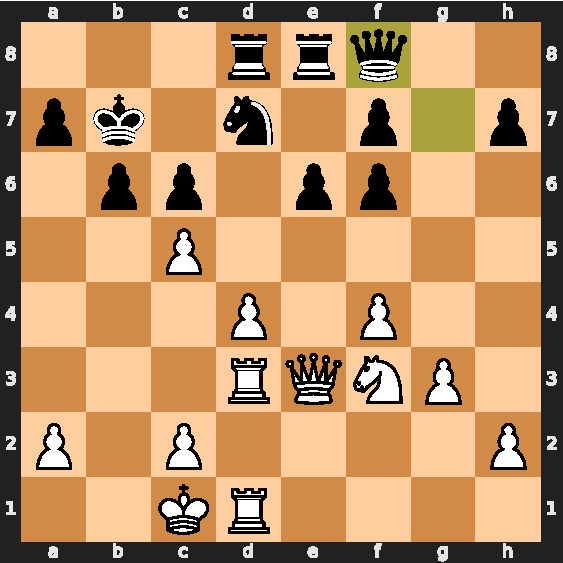
\includegraphics[width=\boardwidth]{diagrams/board-caa03a4ecc25}}}

\Move{\href{https://lichess.org/analysis/pgn/d4_e6_e4_d5_Nc3_Nf6_Bg5_Bb4_exd5_Qxd5_Bxf6_Bxc3_bxc3_gxf6_Nf3_b6_Qd2_Bb7_Be2_Nd7_c4_Qf5_O-O-O_O-O-O_Qe3_Rhg8_g3_Qa5_Rd3_Kb8_Rhd1_Qf5_Nh4_Qg5_f4_Qg7_Bf3_Rge8_Bxb7_Kxb7_c5_c6_Nf3_Qf8_Nd2}{23.\figN d2?}}

I had considered \href{https://lichess.org/analysis/pgn/d4_e6_e4_d5_Nc3_Nf6_Bg5_Bb4_exd5_Qxd5_Bxf6_Bxc3_bxc3_gxf6_Nf3_b6_Qd2_Bb7_Be2_Nd7_c4_Qf5_O-O-O_O-O-O_Qe3_Rhg8_g3_Qa5_Rd3_Kb8_Rhd1_Qf5_Nh4_Qg5_f4_Qg7_Bf3_Rge8_Bxb7_Kxb7_c5_c6_Nf3_Qf8_Rb3}{23.\figR b3}, which was the right move, but gave it up because it seemed too slow, and that in such a position there had to be some quicker way of winning.

\Move{\href{https://lichess.org/analysis/pgn/d4_e6_e4_d5_Nc3_Nf6_Bg5_Bb4_exd5_Qxd5_Bxf6_Bxc3_bxc3_gxf6_Nf3_b6_Qd2_Bb7_Be2_Nd7_c4_Qf5_O-O-O_O-O-O_Qe3_Rhg8_g3_Qa5_Rd3_Kb8_Rhd1_Qf5_Nh4_Qg5_f4_Qg7_Bf3_Rge8_Bxb7_Kxb7_c5_c6_Nf3_Qf8_Nd2_bxc5}{23...bxc5} \href{https://lichess.org/analysis/pgn/d4_e6_e4_d5_Nc3_Nf6_Bg5_Bb4_exd5_Qxd5_Bxf6_Bxc3_bxc3_gxf6_Nf3_b6_Qd2_Bb7_Be2_Nd7_c4_Qf5_O-O-O_O-O-O_Qe3_Rhg8_g3_Qa5_Rd3_Kb8_Rhd1_Qf5_Nh4_Qg5_f4_Qg7_Bf3_Rge8_Bxb7_Kxb7_c5_c6_Nf3_Qf8_Nd2_bxc5_Nc4}{24.\figN c4}}

\href{https://lichess.org/analysis/pgn/d4_e6_e4_d5_Nc3_Nf6_Bg5_Bb4_exd5_Qxd5_Bxf6_Bxc3_bxc3_gxf6_Nf3_b6_Qd2_Bb7_Be2_Nd7_c4_Qf5_O-O-O_O-O-O_Qe3_Rhg8_g3_Qa5_Rd3_Kb8_Rhd1_Qf5_Nh4_Qg5_f4_Qg7_Bf3_Rge8_Bxb7_Kxb7_c5_c6_Nf3_Qf8_Nd2_bxc5_Ne4}{24.\figN e4} or \href{https://lichess.org/analysis/pgn/d4_e6_e4_d5_Nc3_Nf6_Bg5_Bb4_exd5_Qxd5_Bxf6_Bxc3_bxc3_gxf6_Nf3_b6_Qd2_Bb7_Be2_Nd7_c4_Qf5_O-O-O_O-O-O_Qe3_Rhg8_g3_Qa5_Rd3_Kb8_Rhd1_Qf5_Nh4_Qg5_f4_Qg7_Bf3_Rge8_Bxb7_Kxb7_c5_c6_Nf3_Qf8_Nd2_bxc5_Nb3}{24.\figN b3} would have brought about an ending advantageous to White.

\Move{\href{https://lichess.org/analysis/pgn/d4_e6_e4_d5_Nc3_Nf6_Bg5_Bb4_exd5_Qxd5_Bxf6_Bxc3_bxc3_gxf6_Nf3_b6_Qd2_Bb7_Be2_Nd7_c4_Qf5_O-O-O_O-O-O_Qe3_Rhg8_g3_Qa5_Rd3_Kb8_Rhd1_Qf5_Nh4_Qg5_f4_Qg7_Bf3_Rge8_Bxb7_Kxb7_c5_c6_Nf3_Qf8_Nd2_bxc5_Nc4_Nb6}{24...\figN b6} \href{https://lichess.org/analysis/pgn/d4_e6_e4_d5_Nc3_Nf6_Bg5_Bb4_exd5_Qxd5_Bxf6_Bxc3_bxc3_gxf6_Nf3_b6_Qd2_Bb7_Be2_Nd7_c4_Qf5_O-O-O_O-O-O_Qe3_Rhg8_g3_Qa5_Rd3_Kb8_Rhd1_Qf5_Nh4_Qg5_f4_Qg7_Bf3_Rge8_Bxb7_Kxb7_c5_c6_Nf3_Qf8_Nd2_bxc5_Nc4_Nb6_Na5}{25.\figN a5+} \href{https://lichess.org/analysis/pgn/d4_e6_e4_d5_Nc3_Nf6_Bg5_Bb4_exd5_Qxd5_Bxf6_Bxc3_bxc3_gxf6_Nf3_b6_Qd2_Bb7_Be2_Nd7_c4_Qf5_O-O-O_O-O-O_Qe3_Rhg8_g3_Qa5_Rd3_Kb8_Rhd1_Qf5_Nh4_Qg5_f4_Qg7_Bf3_Rge8_Bxb7_Kxb7_c5_c6_Nf3_Qf8_Nd2_bxc5_Nc4_Nb6_Na5_Ka8}{\figK a8} \href{https://lichess.org/analysis/pgn/d4_e6_e4_d5_Nc3_Nf6_Bg5_Bb4_exd5_Qxd5_Bxf6_Bxc3_bxc3_gxf6_Nf3_b6_Qd2_Bb7_Be2_Nd7_c4_Qf5_O-O-O_O-O-O_Qe3_Rhg8_g3_Qa5_Rd3_Kb8_Rhd1_Qf5_Nh4_Qg5_f4_Qg7_Bf3_Rge8_Bxb7_Kxb7_c5_c6_Nf3_Qf8_Nd2_bxc5_Nc4_Nb6_Na5_Ka8_dxc5}{26.dxc5} \href{https://lichess.org/analysis/pgn/d4_e6_e4_d5_Nc3_Nf6_Bg5_Bb4_exd5_Qxd5_Bxf6_Bxc3_bxc3_gxf6_Nf3_b6_Qd2_Bb7_Be2_Nd7_c4_Qf5_O-O-O_O-O-O_Qe3_Rhg8_g3_Qa5_Rd3_Kb8_Rhd1_Qf5_Nh4_Qg5_f4_Qg7_Bf3_Rge8_Bxb7_Kxb7_c5_c6_Nf3_Qf8_Nd2_bxc5_Nc4_Nb6_Na5_Ka8_dxc5_Nd5}{\figN d5} \href{https://lichess.org/analysis/pgn/d4_e6_e4_d5_Nc3_Nf6_Bg5_Bb4_exd5_Qxd5_Bxf6_Bxc3_bxc3_gxf6_Nf3_b6_Qd2_Bb7_Be2_Nd7_c4_Qf5_O-O-O_O-O-O_Qe3_Rhg8_g3_Qa5_Rd3_Kb8_Rhd1_Qf5_Nh4_Qg5_f4_Qg7_Bf3_Rge8_Bxb7_Kxb7_c5_c6_Nf3_Qf8_Nd2_bxc5_Nc4_Nb6_Na5_Ka8_dxc5_Nd5_Qd4}{27.\figQ d4} \href{https://lichess.org/analysis/pgn/d4_e6_e4_d5_Nc3_Nf6_Bg5_Bb4_exd5_Qxd5_Bxf6_Bxc3_bxc3_gxf6_Nf3_b6_Qd2_Bb7_Be2_Nd7_c4_Qf5_O-O-O_O-O-O_Qe3_Rhg8_g3_Qa5_Rd3_Kb8_Rhd1_Qf5_Nh4_Qg5_f4_Qg7_Bf3_Rge8_Bxb7_Kxb7_c5_c6_Nf3_Qf8_Nd2_bxc5_Nc4_Nb6_Na5_Ka8_dxc5_Nd5_Qd4_Rc8}{\figR c8}}

If \href{https://lichess.org/analysis/pgn/d4_e6_e4_d5_Nc3_Nf6_Bg5_Bb4_exd5_Qxd5_Bxf6_Bxc3_bxc3_gxf6_Nf3_b6_Qd2_Bb7_Be2_Nd7_c4_Qf5_O-O-O_O-O-O_Qe3_Rhg8_g3_Qa5_Rd3_Kb8_Rhd1_Qf5_Nh4_Qg5_f4_Qg7_Bf3_Rge8_Bxb7_Kxb7_c5_c6_Nf3_Qf8_Nd2_bxc5_Nc4_Nb6_Na5_Ka8_dxc5_Nd5_Qd4_Rb8}{27...\figR b8} \href{https://lichess.org/analysis/pgn/d4_e6_e4_d5_Nc3_Nf6_Bg5_Bb4_exd5_Qxd5_Bxf6_Bxc3_bxc3_gxf6_Nf3_b6_Qd2_Bb7_Be2_Nd7_c4_Qf5_O-O-O_O-O-O_Qe3_Rhg8_g3_Qa5_Rd3_Kb8_Rhd1_Qf5_Nh4_Qg5_f4_Qg7_Bf3_Rge8_Bxb7_Kxb7_c5_c6_Nf3_Qf8_Nd2_bxc5_Nc4_Nb6_Na5_Ka8_dxc5_Nd5_Qd4_Rb8_Nxc6}{28.\figN xc6} \href{https://lichess.org/analysis/pgn/d4_e6_e4_d5_Nc3_Nf6_Bg5_Bb4_exd5_Qxd5_Bxf6_Bxc3_bxc3_gxf6_Nf3_b6_Qd2_Bb7_Be2_Nd7_c4_Qf5_O-O-O_O-O-O_Qe3_Rhg8_g3_Qa5_Rd3_Kb8_Rhd1_Qf5_Nh4_Qg5_f4_Qg7_Bf3_Rge8_Bxb7_Kxb7_c5_c6_Nf3_Qf8_Nd2_bxc5_Nc4_Nb6_Na5_Ka8_dxc5_Nd5_Qd4_Rb8_Nxc6_Rbc8}{\figR bc8} \href{https://lichess.org/analysis/pgn/d4_e6_e4_d5_Nc3_Nf6_Bg5_Bb4_exd5_Qxd5_Bxf6_Bxc3_bxc3_gxf6_Nf3_b6_Qd2_Bb7_Be2_Nd7_c4_Qf5_O-O-O_O-O-O_Qe3_Rhg8_g3_Qa5_Rd3_Kb8_Rhd1_Qf5_Nh4_Qg5_f4_Qg7_Bf3_Rge8_Bxb7_Kxb7_c5_c6_Nf3_Qf8_Nd2_bxc5_Nc4_Nb6_Na5_Ka8_dxc5_Nd5_Qd4_Rb8_Nxc6_Rbc8_Nxa7}{29.\figN xa7} would win.

\ChessDiagram{\href{https://lichess.org/analysis/pgn/d4_e6_e4_d5_Nc3_Nf6_Bg5_Bb4_exd5_Qxd5_Bxf6_Bxc3_bxc3_gxf6_Nf3_b6_Qd2_Bb7_Be2_Nd7_c4_Qf5_O-O-O_O-O-O_Qe3_Rhg8_g3_Qa5_Rd3_Kb8_Rhd1_Qf5_Nh4_Qg5_f4_Qg7_Bf3_Rge8_Bxb7_Kxb7_c5_c6_Nf3_Qf8_Nd2_bxc5_Nc4_Nb6_Na5_Ka8_dxc5_Nd5_Qd4_Rc8}{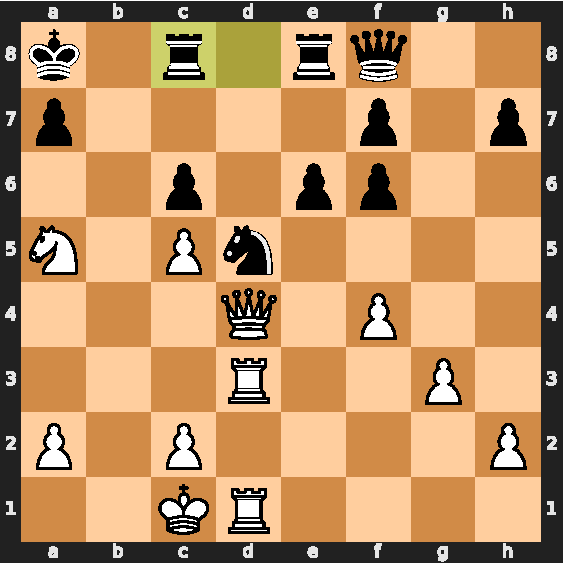
\includegraphics[width=\boardwidth]{diagrams/board-51055049396e}}}

\Move{\href{https://lichess.org/analysis/pgn/d4_e6_e4_d5_Nc3_Nf6_Bg5_Bb4_exd5_Qxd5_Bxf6_Bxc3_bxc3_gxf6_Nf3_b6_Qd2_Bb7_Be2_Nd7_c4_Qf5_O-O-O_O-O-O_Qe3_Rhg8_g3_Qa5_Rd3_Kb8_Rhd1_Qf5_Nh4_Qg5_f4_Qg7_Bf3_Rge8_Bxb7_Kxb7_c5_c6_Nf3_Qf8_Nd2_bxc5_Nc4_Nb6_Na5_Ka8_dxc5_Nd5_Qd4_Rc8_c4}{28.c4}}

\href{https://lichess.org/analysis/pgn/d4_e6_e4_d5_Nc3_Nf6_Bg5_Bb4_exd5_Qxd5_Bxf6_Bxc3_bxc3_gxf6_Nf3_b6_Qd2_Bb7_Be2_Nd7_c4_Qf5_O-O-O_O-O-O_Qe3_Rhg8_g3_Qa5_Rd3_Kb8_Rhd1_Qf5_Nh4_Qg5_f4_Qg7_Bf3_Rge8_Bxb7_Kxb7_c5_c6_Nf3_Qf8_Nd2_bxc5_Nc4_Nb6_Na5_Ka8_dxc5_Nd5_Qd4_Rc8_Nc4}{28.\figN c4} was the right move. I was, however, still looking for the ``grand combination,'' and thought that the Pawn I would later on have at d6 would win the game. Black deserves great credit for the way in which he conducted this exceedingly difficult defence. He could easily have gone wrong any number of times, but from move 22 onwards he always played the best move.

\Move{\href{https://lichess.org/analysis/pgn/d4_e6_e4_d5_Nc3_Nf6_Bg5_Bb4_exd5_Qxd5_Bxf6_Bxc3_bxc3_gxf6_Nf3_b6_Qd2_Bb7_Be2_Nd7_c4_Qf5_O-O-O_O-O-O_Qe3_Rhg8_g3_Qa5_Rd3_Kb8_Rhd1_Qf5_Nh4_Qg5_f4_Qg7_Bf3_Rge8_Bxb7_Kxb7_c5_c6_Nf3_Qf8_Nd2_bxc5_Nc4_Nb6_Na5_Ka8_dxc5_Nd5_Qd4_Rc8_c4_e5}{28...e5!} \href{https://lichess.org/analysis/pgn/d4_e6_e4_d5_Nc3_Nf6_Bg5_Bb4_exd5_Qxd5_Bxf6_Bxc3_bxc3_gxf6_Nf3_b6_Qd2_Bb7_Be2_Nd7_c4_Qf5_O-O-O_O-O-O_Qe3_Rhg8_g3_Qa5_Rd3_Kb8_Rhd1_Qf5_Nh4_Qg5_f4_Qg7_Bf3_Rge8_Bxb7_Kxb7_c5_c6_Nf3_Qf8_Nd2_bxc5_Nc4_Nb6_Na5_Ka8_dxc5_Nd5_Qd4_Rc8_c4_e5_Qg1}{29.\figQ g1} \href{https://lichess.org/analysis/pgn/d4_e6_e4_d5_Nc3_Nf6_Bg5_Bb4_exd5_Qxd5_Bxf6_Bxc3_bxc3_gxf6_Nf3_b6_Qd2_Bb7_Be2_Nd7_c4_Qf5_O-O-O_O-O-O_Qe3_Rhg8_g3_Qa5_Rd3_Kb8_Rhd1_Qf5_Nh4_Qg5_f4_Qg7_Bf3_Rge8_Bxb7_Kxb7_c5_c6_Nf3_Qf8_Nd2_bxc5_Nc4_Nb6_Na5_Ka8_dxc5_Nd5_Qd4_Rc8_c4_e5_Qg1_e4}{e4} \href{https://lichess.org/analysis/pgn/d4_e6_e4_d5_Nc3_Nf6_Bg5_Bb4_exd5_Qxd5_Bxf6_Bxc3_bxc3_gxf6_Nf3_b6_Qd2_Bb7_Be2_Nd7_c4_Qf5_O-O-O_O-O-O_Qe3_Rhg8_g3_Qa5_Rd3_Kb8_Rhd1_Qf5_Nh4_Qg5_f4_Qg7_Bf3_Rge8_Bxb7_Kxb7_c5_c6_Nf3_Qf8_Nd2_bxc5_Nc4_Nb6_Na5_Ka8_dxc5_Nd5_Qd4_Rc8_c4_e5_Qg1_e4_cxd5}{30.cxd5} \href{https://lichess.org/analysis/pgn/d4_e6_e4_d5_Nc3_Nf6_Bg5_Bb4_exd5_Qxd5_Bxf6_Bxc3_bxc3_gxf6_Nf3_b6_Qd2_Bb7_Be2_Nd7_c4_Qf5_O-O-O_O-O-O_Qe3_Rhg8_g3_Qa5_Rd3_Kb8_Rhd1_Qf5_Nh4_Qg5_f4_Qg7_Bf3_Rge8_Bxb7_Kxb7_c5_c6_Nf3_Qf8_Nd2_bxc5_Nc4_Nb6_Na5_Ka8_dxc5_Nd5_Qd4_Rc8_c4_e5_Qg1_e4_cxd5_exd3}{exd3} \href{https://lichess.org/analysis/pgn/d4_e6_e4_d5_Nc3_Nf6_Bg5_Bb4_exd5_Qxd5_Bxf6_Bxc3_bxc3_gxf6_Nf3_b6_Qd2_Bb7_Be2_Nd7_c4_Qf5_O-O-O_O-O-O_Qe3_Rhg8_g3_Qa5_Rd3_Kb8_Rhd1_Qf5_Nh4_Qg5_f4_Qg7_Bf3_Rge8_Bxb7_Kxb7_c5_c6_Nf3_Qf8_Nd2_bxc5_Nc4_Nb6_Na5_Ka8_dxc5_Nd5_Qd4_Rc8_c4_e5_Qg1_e4_cxd5_exd3_d6}{31.d6} \href{https://lichess.org/analysis/pgn/d4_e6_e4_d5_Nc3_Nf6_Bg5_Bb4_exd5_Qxd5_Bxf6_Bxc3_bxc3_gxf6_Nf3_b6_Qd2_Bb7_Be2_Nd7_c4_Qf5_O-O-O_O-O-O_Qe3_Rhg8_g3_Qa5_Rd3_Kb8_Rhd1_Qf5_Nh4_Qg5_f4_Qg7_Bf3_Rge8_Bxb7_Kxb7_c5_c6_Nf3_Qf8_Nd2_bxc5_Nc4_Nb6_Na5_Ka8_dxc5_Nd5_Qd4_Rc8_c4_e5_Qg1_e4_cxd5_exd3_d6_Re2}{\figR e2} \href{https://lichess.org/analysis/pgn/d4_e6_e4_d5_Nc3_Nf6_Bg5_Bb4_exd5_Qxd5_Bxf6_Bxc3_bxc3_gxf6_Nf3_b6_Qd2_Bb7_Be2_Nd7_c4_Qf5_O-O-O_O-O-O_Qe3_Rhg8_g3_Qa5_Rd3_Kb8_Rhd1_Qf5_Nh4_Qg5_f4_Qg7_Bf3_Rge8_Bxb7_Kxb7_c5_c6_Nf3_Qf8_Nd2_bxc5_Nc4_Nb6_Na5_Ka8_dxc5_Nd5_Qd4_Rc8_c4_e5_Qg1_e4_cxd5_exd3_d6_Re2_d7}{32.d7} \href{https://lichess.org/analysis/pgn/d4_e6_e4_d5_Nc3_Nf6_Bg5_Bb4_exd5_Qxd5_Bxf6_Bxc3_bxc3_gxf6_Nf3_b6_Qd2_Bb7_Be2_Nd7_c4_Qf5_O-O-O_O-O-O_Qe3_Rhg8_g3_Qa5_Rd3_Kb8_Rhd1_Qf5_Nh4_Qg5_f4_Qg7_Bf3_Rge8_Bxb7_Kxb7_c5_c6_Nf3_Qf8_Nd2_bxc5_Nc4_Nb6_Na5_Ka8_dxc5_Nd5_Qd4_Rc8_c4_e5_Qg1_e4_cxd5_exd3_d6_Re2_d7_Rc2}{\figR c2+} \href{https://lichess.org/analysis/pgn/d4_e6_e4_d5_Nc3_Nf6_Bg5_Bb4_exd5_Qxd5_Bxf6_Bxc3_bxc3_gxf6_Nf3_b6_Qd2_Bb7_Be2_Nd7_c4_Qf5_O-O-O_O-O-O_Qe3_Rhg8_g3_Qa5_Rd3_Kb8_Rhd1_Qf5_Nh4_Qg5_f4_Qg7_Bf3_Rge8_Bxb7_Kxb7_c5_c6_Nf3_Qf8_Nd2_bxc5_Nc4_Nb6_Na5_Ka8_dxc5_Nd5_Qd4_Rc8_c4_e5_Qg1_e4_cxd5_exd3_d6_Re2_d7_Rc2_Kb1}{33.\figK b1} \href{https://lichess.org/analysis/pgn/d4_e6_e4_d5_Nc3_Nf6_Bg5_Bb4_exd5_Qxd5_Bxf6_Bxc3_bxc3_gxf6_Nf3_b6_Qd2_Bb7_Be2_Nd7_c4_Qf5_O-O-O_O-O-O_Qe3_Rhg8_g3_Qa5_Rd3_Kb8_Rhd1_Qf5_Nh4_Qg5_f4_Qg7_Bf3_Rge8_Bxb7_Kxb7_c5_c6_Nf3_Qf8_Nd2_bxc5_Nc4_Nb6_Na5_Ka8_dxc5_Nd5_Qd4_Rc8_c4_e5_Qg1_e4_cxd5_exd3_d6_Re2_d7_Rc2_Kb1_Rb8}{\figR b8+} \href{https://lichess.org/analysis/pgn/d4_e6_e4_d5_Nc3_Nf6_Bg5_Bb4_exd5_Qxd5_Bxf6_Bxc3_bxc3_gxf6_Nf3_b6_Qd2_Bb7_Be2_Nd7_c4_Qf5_O-O-O_O-O-O_Qe3_Rhg8_g3_Qa5_Rd3_Kb8_Rhd1_Qf5_Nh4_Qg5_f4_Qg7_Bf3_Rge8_Bxb7_Kxb7_c5_c6_Nf3_Qf8_Nd2_bxc5_Nc4_Nb6_Na5_Ka8_dxc5_Nd5_Qd4_Rc8_c4_e5_Qg1_e4_cxd5_exd3_d6_Re2_d7_Rc2_Kb1_Rb8_Nb3}{34.\figN b3} \href{https://lichess.org/analysis/pgn/d4_e6_e4_d5_Nc3_Nf6_Bg5_Bb4_exd5_Qxd5_Bxf6_Bxc3_bxc3_gxf6_Nf3_b6_Qd2_Bb7_Be2_Nd7_c4_Qf5_O-O-O_O-O-O_Qe3_Rhg8_g3_Qa5_Rd3_Kb8_Rhd1_Qf5_Nh4_Qg5_f4_Qg7_Bf3_Rge8_Bxb7_Kxb7_c5_c6_Nf3_Qf8_Nd2_bxc5_Nc4_Nb6_Na5_Ka8_dxc5_Nd5_Qd4_Rc8_c4_e5_Qg1_e4_cxd5_exd3_d6_Re2_d7_Rc2_Kb1_Rb8_Nb3_Qe7}{\figQ e7}}

\ChessDiagram{\href{https://lichess.org/analysis/pgn/d4_e6_e4_d5_Nc3_Nf6_Bg5_Bb4_exd5_Qxd5_Bxf6_Bxc3_bxc3_gxf6_Nf3_b6_Qd2_Bb7_Be2_Nd7_c4_Qf5_O-O-O_O-O-O_Qe3_Rhg8_g3_Qa5_Rd3_Kb8_Rhd1_Qf5_Nh4_Qg5_f4_Qg7_Bf3_Rge8_Bxb7_Kxb7_c5_c6_Nf3_Qf8_Nd2_bxc5_Nc4_Nb6_Na5_Ka8_dxc5_Nd5_Qd4_Rc8_c4_e5_Qg1_e4_cxd5_exd3_d6_Re2_d7_Rc2_Kb1_Rb8_Nb3_Qe7}{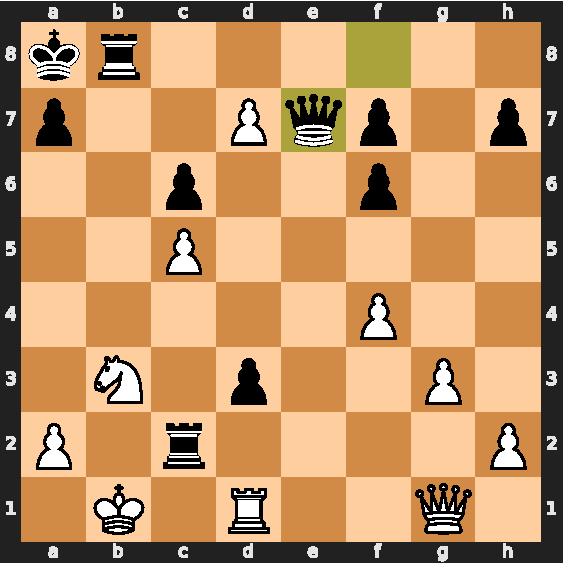
\includegraphics[width=\boardwidth]{diagrams/board-6a4ea48911b2}}}

\Move{\href{https://lichess.org/analysis/pgn/d4_e6_e4_d5_Nc3_Nf6_Bg5_Bb4_exd5_Qxd5_Bxf6_Bxc3_bxc3_gxf6_Nf3_b6_Qd2_Bb7_Be2_Nd7_c4_Qf5_O-O-O_O-O-O_Qe3_Rhg8_g3_Qa5_Rd3_Kb8_Rhd1_Qf5_Nh4_Qg5_f4_Qg7_Bf3_Rge8_Bxb7_Kxb7_c5_c6_Nf3_Qf8_Nd2_bxc5_Nc4_Nb6_Na5_Ka8_dxc5_Nd5_Qd4_Rc8_c4_e5_Qg1_e4_cxd5_exd3_d6_Re2_d7_Rc2_Kb1_Rb8_Nb3_Qe7_Rxd3}{35.\figR xd3}}

The position is most interesting. I believe I lost here my last chance to win the game, and if that is true it would vindicate my judgment when, on move 28, I played \href{https://lichess.org/analysis/pgn/d4_e6_e4_d5_Nc3_Nf6_Bg5_Bb4_exd5_Qxd5_Bxf6_Bxc3_bxc3_gxf6_Nf3_b6_Qd2_Bb7_Be2_Nd7_c4_Qf5_O-O-O_O-O-O_Qe3_Rhg8_g3_Qa5_Rd3_Kb8_Rhd1_Qf5_Nh4_Qg5_f4_Qg7_Bf3_Rge8_Bxb7_Kxb7_c5_c6_Nf3_Qf8_Nd2_bxc5_Nc4_Nb6_Na5_Ka8_dxc5_Nd5_Qd4_Rc8_c4}{28.c4}. The student can find out what would happen if White plays \href{https://lichess.org/analysis/pgn/d4_e6_e4_d5_Nc3_Nf6_Bg5_Bb4_exd5_Qxd5_Bxf6_Bxc3_bxc3_gxf6_Nf3_b6_Qd2_Bb7_Be2_Nd7_c4_Qf5_O-O-O_O-O-O_Qe3_Rhg8_g3_Qa5_Rd3_Kb8_Rhd1_Qf5_Nh4_Qg5_f4_Qg7_Bf3_Rge8_Bxb7_Kxb7_c5_c6_Nf3_Qf8_Nd2_bxc5_Nc4_Nb6_Na5_Ka8_dxc5_Nd5_Qd4_Rc8_c4_e5_Qg1_e4_cxd5_exd3_d6_Re2_d7_Rc2_Kb1_Rb8_Nb3_Qe7_Qd4}{35.\figQ d4!} at once. I have gone over the following variations: \href{https://lichess.org/analysis/pgn/d4_e6_e4_d5_Nc3_Nf6_Bg5_Bb4_exd5_Qxd5_Bxf6_Bxc3_bxc3_gxf6_Nf3_b6_Qd2_Bb7_Be2_Nd7_c4_Qf5_O-O-O_O-O-O_Qe3_Rhg8_g3_Qa5_Rd3_Kb8_Rhd1_Qf5_Nh4_Qg5_f4_Qg7_Bf3_Rge8_Bxb7_Kxb7_c5_c6_Nf3_Qf8_Nd2_bxc5_Nc4_Nb6_Na5_Ka8_dxc5_Nd5_Qd4_Rc8_c4_e5_Qg1_e4_cxd5_exd3_d6_Re2_d7_Rc2_Kb1_Rb8_Nb3_Qe7_Qd4}{35.\figQ d4}, \href{https://lichess.org/analysis/pgn/d4_e6_e4_d5_Nc3_Nf6_Bg5_Bb4_exd5_Qxd5_Bxf6_Bxc3_bxc3_gxf6_Nf3_b6_Qd2_Bb7_Be2_Nd7_c4_Qf5_O-O-O_O-O-O_Qe3_Rhg8_g3_Qa5_Rd3_Kb8_Rhd1_Qf5_Nh4_Qg5_f4_Qg7_Bf3_Rge8_Bxb7_Kxb7_c5_c6_Nf3_Qf8_Nd2_bxc5_Nc4_Nb6_Na5_Ka8_dxc5_Nd5_Qd4_Rc8_c4_e5_Qg1_e4_cxd5_exd3_d6_Re2_d7_Rc2_Kb1_Rb8_Nb3_Qe7_Qd4_Rxh2}{35...\figR xh2} (of course if \href{https://lichess.org/analysis/pgn/d4_e6_e4_d5_Nc3_Nf6_Bg5_Bb4_exd5_Qxd5_Bxf6_Bxc3_bxc3_gxf6_Nf3_b6_Qd2_Bb7_Be2_Nd7_c4_Qf5_O-O-O_O-O-O_Qe3_Rhg8_g3_Qa5_Rd3_Kb8_Rhd1_Qf5_Nh4_Qg5_f4_Qg7_Bf3_Rge8_Bxb7_Kxb7_c5_c6_Nf3_Qf8_Nd2_bxc5_Nc4_Nb6_Na5_Ka8_dxc5_Nd5_Qd4_Rc8_c4_e5_Qg1_e4_cxd5_exd3_d6_Re2_d7_Rc2_Kb1_Rb8_Nb3_Qe7_Qd4_Rxc5}{35...\figR xc5} \href{https://lichess.org/analysis/pgn/d4_e6_e4_d5_Nc3_Nf6_Bg5_Bb4_exd5_Qxd5_Bxf6_Bxc3_bxc3_gxf6_Nf3_b6_Qd2_Bb7_Be2_Nd7_c4_Qf5_O-O-O_O-O-O_Qe3_Rhg8_g3_Qa5_Rd3_Kb8_Rhd1_Qf5_Nh4_Qg5_f4_Qg7_Bf3_Rge8_Bxb7_Kxb7_c5_c6_Nf3_Qf8_Nd2_bxc5_Nc4_Nb6_Na5_Ka8_dxc5_Nd5_Qd4_Rc8_c4_e5_Qg1_e4_cxd5_exd3_d6_Re2_d7_Rc2_Kb1_Rb8_Nb3_Qe7_Qd4_Rxc5_d8=Q}{36.d8=Q} wins); \href{https://lichess.org/analysis/pgn/d4_e6_e4_d5_Nc3_Nf6_Bg5_Bb4_exd5_Qxd5_Bxf6_Bxc3_bxc3_gxf6_Nf3_b6_Qd2_Bb7_Be2_Nd7_c4_Qf5_O-O-O_O-O-O_Qe3_Rhg8_g3_Qa5_Rd3_Kb8_Rhd1_Qf5_Nh4_Qg5_f4_Qg7_Bf3_Rge8_Bxb7_Kxb7_c5_c6_Nf3_Qf8_Nd2_bxc5_Nc4_Nb6_Na5_Ka8_dxc5_Nd5_Qd4_Rc8_c4_e5_Qg1_e4_cxd5_exd3_d6_Re2_d7_Rc2_Kb1_Rb8_Nb3_Qe7_Qd4_Rxh2_Qxd3}{36.\figQ xd3!} \href{https://lichess.org/analysis/pgn/d4_e6_e4_d5_Nc3_Nf6_Bg5_Bb4_exd5_Qxd5_Bxf6_Bxc3_bxc3_gxf6_Nf3_b6_Qd2_Bb7_Be2_Nd7_c4_Qf5_O-O-O_O-O-O_Qe3_Rhg8_g3_Qa5_Rd3_Kb8_Rhd1_Qf5_Nh4_Qg5_f4_Qg7_Bf3_Rge8_Bxb7_Kxb7_c5_c6_Nf3_Qf8_Nd2_bxc5_Nc4_Nb6_Na5_Ka8_dxc5_Nd5_Qd4_Rc8_c4_e5_Qg1_e4_cxd5_exd3_d6_Re2_d7_Rc2_Kb1_Rb8_Nb3_Qe7_Qd4_Rxh2_Qxd3_Rd8}{\figR d8} \href{https://lichess.org/analysis/pgn/d4_e6_e4_d5_Nc3_Nf6_Bg5_Bb4_exd5_Qxd5_Bxf6_Bxc3_bxc3_gxf6_Nf3_b6_Qd2_Bb7_Be2_Nd7_c4_Qf5_O-O-O_O-O-O_Qe3_Rhg8_g3_Qa5_Rd3_Kb8_Rhd1_Qf5_Nh4_Qg5_f4_Qg7_Bf3_Rge8_Bxb7_Kxb7_c5_c6_Nf3_Qf8_Nd2_bxc5_Nc4_Nb6_Na5_Ka8_dxc5_Nd5_Qd4_Rc8_c4_e5_Qg1_e4_cxd5_exd3_d6_Re2_d7_Rc2_Kb1_Rb8_Nb3_Qe7_Qd4_Rxh2_Qxd3_Rd8_Qa6}{37.\figQ a6} \href{https://lichess.org/analysis/pgn/d4_e6_e4_d5_Nc3_Nf6_Bg5_Bb4_exd5_Qxd5_Bxf6_Bxc3_bxc3_gxf6_Nf3_b6_Qd2_Bb7_Be2_Nd7_c4_Qf5_O-O-O_O-O-O_Qe3_Rhg8_g3_Qa5_Rd3_Kb8_Rhd1_Qf5_Nh4_Qg5_f4_Qg7_Bf3_Rge8_Bxb7_Kxb7_c5_c6_Nf3_Qf8_Nd2_bxc5_Nc4_Nb6_Na5_Ka8_dxc5_Nd5_Qd4_Rc8_c4_e5_Qg1_e4_cxd5_exd3_d6_Re2_d7_Rc2_Kb1_Rb8_Nb3_Qe7_Qd4_Rxh2_Qxd3_Rd8_Qa6_Kb8}{\figK b8} best (if \figQ d4+; \figK a1, \figK b8; \figR b1 wins); \href{https://lichess.org/analysis/pgn/d4_e6_e4_d5_Nc3_Nf6_Bg5_Bb4_exd5_Qxd5_Bxf6_Bxc3_bxc3_gxf6_Nf3_b6_Qd2_Bb7_Be2_Nd7_c4_Qf5_O-O-O_O-O-O_Qe3_Rhg8_g3_Qa5_Rd3_Kb8_Rhd1_Qf5_Nh4_Qg5_f4_Qg7_Bf3_Rge8_Bxb7_Kxb7_c5_c6_Nf3_Qf8_Nd2_bxc5_Nc4_Nb6_Na5_Ka8_dxc5_Nd5_Qd4_Rc8_c4_e5_Qg1_e4_cxd5_exd3_d6_Re2_d7_Rc2_Kb1_Rb8_Nb3_Qe7_Qd4_Rxh2_Qxd3_Rd8_Qa6_Kb8_Qxc6}{38.\figQ xc6} and White will at least have a draw.

\Move{\href{https://lichess.org/analysis/pgn/d4_e6_e4_d5_Nc3_Nf6_Bg5_Bb4_exd5_Qxd5_Bxf6_Bxc3_bxc3_gxf6_Nf3_b6_Qd2_Bb7_Be2_Nd7_c4_Qf5_O-O-O_O-O-O_Qe3_Rhg8_g3_Qa5_Rd3_Kb8_Rhd1_Qf5_Nh4_Qg5_f4_Qg7_Bf3_Rge8_Bxb7_Kxb7_c5_c6_Nf3_Qf8_Nd2_bxc5_Nc4_Nb6_Na5_Ka8_dxc5_Nd5_Qd4_Rc8_c4_e5_Qg1_e4_cxd5_exd3_d6_Re2_d7_Rc2_Kb1_Rb8_Nb3_Qe7_Rxd3_Re2}{35...\figR e2} \href{https://lichess.org/analysis/pgn/d4_e6_e4_d5_Nc3_Nf6_Bg5_Bb4_exd5_Qxd5_Bxf6_Bxc3_bxc3_gxf6_Nf3_b6_Qd2_Bb7_Be2_Nd7_c4_Qf5_O-O-O_O-O-O_Qe3_Rhg8_g3_Qa5_Rd3_Kb8_Rhd1_Qf5_Nh4_Qg5_f4_Qg7_Bf3_Rge8_Bxb7_Kxb7_c5_c6_Nf3_Qf8_Nd2_bxc5_Nc4_Nb6_Na5_Ka8_dxc5_Nd5_Qd4_Rc8_c4_e5_Qg1_e4_cxd5_exd3_d6_Re2_d7_Rc2_Kb1_Rb8_Nb3_Qe7_Rxd3_Re2_Qd4}{36.\figQ d4} \href{https://lichess.org/analysis/pgn/d4_e6_e4_d5_Nc3_Nf6_Bg5_Bb4_exd5_Qxd5_Bxf6_Bxc3_bxc3_gxf6_Nf3_b6_Qd2_Bb7_Be2_Nd7_c4_Qf5_O-O-O_O-O-O_Qe3_Rhg8_g3_Qa5_Rd3_Kb8_Rhd1_Qf5_Nh4_Qg5_f4_Qg7_Bf3_Rge8_Bxb7_Kxb7_c5_c6_Nf3_Qf8_Nd2_bxc5_Nc4_Nb6_Na5_Ka8_dxc5_Nd5_Qd4_Rc8_c4_e5_Qg1_e4_cxd5_exd3_d6_Re2_d7_Rc2_Kb1_Rb8_Nb3_Qe7_Rxd3_Re2_Qd4_Rd8}{\figR d8} \href{https://lichess.org/analysis/pgn/d4_e6_e4_d5_Nc3_Nf6_Bg5_Bb4_exd5_Qxd5_Bxf6_Bxc3_bxc3_gxf6_Nf3_b6_Qd2_Bb7_Be2_Nd7_c4_Qf5_O-O-O_O-O-O_Qe3_Rhg8_g3_Qa5_Rd3_Kb8_Rhd1_Qf5_Nh4_Qg5_f4_Qg7_Bf3_Rge8_Bxb7_Kxb7_c5_c6_Nf3_Qf8_Nd2_bxc5_Nc4_Nb6_Na5_Ka8_dxc5_Nd5_Qd4_Rc8_c4_e5_Qg1_e4_cxd5_exd3_d6_Re2_d7_Rc2_Kb1_Rb8_Nb3_Qe7_Rxd3_Re2_Qd4_Rd8_Qa4}{37.\figQ a4} \href{https://lichess.org/analysis/pgn/d4_e6_e4_d5_Nc3_Nf6_Bg5_Bb4_exd5_Qxd5_Bxf6_Bxc3_bxc3_gxf6_Nf3_b6_Qd2_Bb7_Be2_Nd7_c4_Qf5_O-O-O_O-O-O_Qe3_Rhg8_g3_Qa5_Rd3_Kb8_Rhd1_Qf5_Nh4_Qg5_f4_Qg7_Bf3_Rge8_Bxb7_Kxb7_c5_c6_Nf3_Qf8_Nd2_bxc5_Nc4_Nb6_Na5_Ka8_dxc5_Nd5_Qd4_Rc8_c4_e5_Qg1_e4_cxd5_exd3_d6_Re2_d7_Rc2_Kb1_Rb8_Nb3_Qe7_Rxd3_Re2_Qd4_Rd8_Qa4_Qe4}{\figQ e4} \href{https://lichess.org/analysis/pgn/d4_e6_e4_d5_Nc3_Nf6_Bg5_Bb4_exd5_Qxd5_Bxf6_Bxc3_bxc3_gxf6_Nf3_b6_Qd2_Bb7_Be2_Nd7_c4_Qf5_O-O-O_O-O-O_Qe3_Rhg8_g3_Qa5_Rd3_Kb8_Rhd1_Qf5_Nh4_Qg5_f4_Qg7_Bf3_Rge8_Bxb7_Kxb7_c5_c6_Nf3_Qf8_Nd2_bxc5_Nc4_Nb6_Na5_Ka8_dxc5_Nd5_Qd4_Rc8_c4_e5_Qg1_e4_cxd5_exd3_d6_Re2_d7_Rc2_Kb1_Rb8_Nb3_Qe7_Rxd3_Re2_Qd4_Rd8_Qa4_Qe4_Qa6}{38.\figQ a6} \href{https://lichess.org/analysis/pgn/d4_e6_e4_d5_Nc3_Nf6_Bg5_Bb4_exd5_Qxd5_Bxf6_Bxc3_bxc3_gxf6_Nf3_b6_Qd2_Bb7_Be2_Nd7_c4_Qf5_O-O-O_O-O-O_Qe3_Rhg8_g3_Qa5_Rd3_Kb8_Rhd1_Qf5_Nh4_Qg5_f4_Qg7_Bf3_Rge8_Bxb7_Kxb7_c5_c6_Nf3_Qf8_Nd2_bxc5_Nc4_Nb6_Na5_Ka8_dxc5_Nd5_Qd4_Rc8_c4_e5_Qg1_e4_cxd5_exd3_d6_Re2_d7_Rc2_Kb1_Rb8_Nb3_Qe7_Rxd3_Re2_Qd4_Rd8_Qa4_Qe4_Qa6_Kb8}{\figK b8}}

There is nothing to be done against this simple move, since White cannot play \href{https://lichess.org/analysis/pgn/d4_e6_e4_d5_Nc3_Nf6_Bg5_Bb4_exd5_Qxd5_Bxf6_Bxc3_bxc3_gxf6_Nf3_b6_Qd2_Bb7_Be2_Nd7_c4_Qf5_O-O-O_O-O-O_Qe3_Rhg8_g3_Qa5_Rd3_Kb8_Rhd1_Qf5_Nh4_Qg5_f4_Qg7_Bf3_Rge8_Bxb7_Kxb7_c5_c6_Nf3_Qf8_Nd2_bxc5_Nc4_Nb6_Na5_Ka8_dxc5_Nd5_Qd4_Rc8_c4_e5_Qg1_e4_cxd5_exd3_d6_Re2_d7_Rc2_Kb1_Rb8_Nb3_Qe7_Rxd3_Re2_Qd4_Rd8_Qa4_Qe4_Qa6_Kb8_Nd4}{39.\figN d4}, because \href{https://lichess.org/analysis/pgn/d4_e6_e4_d5_Nc3_Nf6_Bg5_Bb4_exd5_Qxd5_Bxf6_Bxc3_bxc3_gxf6_Nf3_b6_Qd2_Bb7_Be2_Nd7_c4_Qf5_O-O-O_O-O-O_Qe3_Rhg8_g3_Qa5_Rd3_Kb8_Rhd1_Qf5_Nh4_Qg5_f4_Qg7_Bf3_Rge8_Bxb7_Kxb7_c5_c6_Nf3_Qf8_Nd2_bxc5_Nc4_Nb6_Na5_Ka8_dxc5_Nd5_Qd4_Rc8_c4_e5_Qg1_e4_cxd5_exd3_d6_Re2_d7_Rc2_Kb1_Rb8_Nb3_Qe7_Rxd3_Re2_Qd4_Rd8_Qa4_Qe4_Qa6_Kb8_Nd4_Qh1}{39...\figQ h1+} mates.

\Move{\href{https://lichess.org/analysis/pgn/d4_e6_e4_d5_Nc3_Nf6_Bg5_Bb4_exd5_Qxd5_Bxf6_Bxc3_bxc3_gxf6_Nf3_b6_Qd2_Bb7_Be2_Nd7_c4_Qf5_O-O-O_O-O-O_Qe3_Rhg8_g3_Qa5_Rd3_Kb8_Rhd1_Qf5_Nh4_Qg5_f4_Qg7_Bf3_Rge8_Bxb7_Kxb7_c5_c6_Nf3_Qf8_Nd2_bxc5_Nc4_Nb6_Na5_Ka8_dxc5_Nd5_Qd4_Rc8_c4_e5_Qg1_e4_cxd5_exd3_d6_Re2_d7_Rc2_Kb1_Rb8_Nb3_Qe7_Rxd3_Re2_Qd4_Rd8_Qa4_Qe4_Qa6_Kb8_Kc1}{39.\figK c1} \href{https://lichess.org/analysis/pgn/d4_e6_e4_d5_Nc3_Nf6_Bg5_Bb4_exd5_Qxd5_Bxf6_Bxc3_bxc3_gxf6_Nf3_b6_Qd2_Bb7_Be2_Nd7_c4_Qf5_O-O-O_O-O-O_Qe3_Rhg8_g3_Qa5_Rd3_Kb8_Rhd1_Qf5_Nh4_Qg5_f4_Qg7_Bf3_Rge8_Bxb7_Kxb7_c5_c6_Nf3_Qf8_Nd2_bxc5_Nc4_Nb6_Na5_Ka8_dxc5_Nd5_Qd4_Rc8_c4_e5_Qg1_e4_cxd5_exd3_d6_Re2_d7_Rc2_Kb1_Rb8_Nb3_Qe7_Rxd3_Re2_Qd4_Rd8_Qa4_Qe4_Qa6_Kb8_Kc1_Rxd7}{\figR xd7} \href{https://lichess.org/analysis/pgn/d4_e6_e4_d5_Nc3_Nf6_Bg5_Bb4_exd5_Qxd5_Bxf6_Bxc3_bxc3_gxf6_Nf3_b6_Qd2_Bb7_Be2_Nd7_c4_Qf5_O-O-O_O-O-O_Qe3_Rhg8_g3_Qa5_Rd3_Kb8_Rhd1_Qf5_Nh4_Qg5_f4_Qg7_Bf3_Rge8_Bxb7_Kxb7_c5_c6_Nf3_Qf8_Nd2_bxc5_Nc4_Nb6_Na5_Ka8_dxc5_Nd5_Qd4_Rc8_c4_e5_Qg1_e4_cxd5_exd3_d6_Re2_d7_Rc2_Kb1_Rb8_Nb3_Qe7_Rxd3_Re2_Qd4_Rd8_Qa4_Qe4_Qa6_Kb8_Kc1_Rxd7_Nd4}{40.\figN d4} \href{https://lichess.org/analysis/pgn/d4_e6_e4_d5_Nc3_Nf6_Bg5_Bb4_exd5_Qxd5_Bxf6_Bxc3_bxc3_gxf6_Nf3_b6_Qd2_Bb7_Be2_Nd7_c4_Qf5_O-O-O_O-O-O_Qe3_Rhg8_g3_Qa5_Rd3_Kb8_Rhd1_Qf5_Nh4_Qg5_f4_Qg7_Bf3_Rge8_Bxb7_Kxb7_c5_c6_Nf3_Qf8_Nd2_bxc5_Nc4_Nb6_Na5_Ka8_dxc5_Nd5_Qd4_Rc8_c4_e5_Qg1_e4_cxd5_exd3_d6_Re2_d7_Rc2_Kb1_Rb8_Nb3_Qe7_Rxd3_Re2_Qd4_Rd8_Qa4_Qe4_Qa6_Kb8_Kc1_Rxd7_Nd4_Re1}{\figR e1+}}

\noindent\textbf{Resigns.}

A very interesting battle.

\end{document}
